% Created 2011-08-22 Mon 11:27
\documentclass[11pt]{article}
%\usepackage[utf8]{inputenc}
\usepackage[T1]{fontenc}
\usepackage{graphicx}
\usepackage{longtable}
\usepackage{hyperref}
\usepackage{comment}
\usepackage{booktabs}
\usepackage{color}
\usepackage{pgf}
\usepackage{tikz}
\usetikzlibrary{arrows,positioning,fit,shapes,decorations,decorations.pathmorphing,decorations.pathreplacing,calc,patterns,scopes,matrix}
\pgfrealjobname{spi}
 
\usepackage{helvet}
\usepackage{enumitem}
\usepackage[letterpaper]{geometry}
\usepackage{listings}
\usepackage{verbatim}
\usepackage[T1]{fontenc}

\setlength{\parindent}{0.0in}
\setlength{\parskip}{0.1in}

\newenvironment{apient}{\small\verbatim}{\endverbatim}

\newcommand{\apidesc}[1]{%
{\addtolength{\leftskip}{4em}%
#1\par\medskip}
}

\begin{document}
\thispagestyle{empty}

\begin{titlepage}
\beginpgfgraphicnamed{titlepage}
\begin{tikzpicture}[remember picture, overlay]
    \path
        (current page.north west) coordinate (origin)
        (current page.north) coordinate (topcenter);

    % Header
    \node [font=\sffamily] (pppt) at ($(topcenter) - (0,1.0in)$) 
        {\fontsize{24}{36}\selectfont Paradyn Parallel Performance Tools};

    % Document Title
% older versions of pgf have a bug for matrices in overlay mode;
% have to specify positions manually
    \matrix (Title) [%
        matrix of nodes,%
        nodes={font=\sffamily,right},%
        matrix anchor=west,%
        row sep=12pt
        ] at ($(origin)+(0.75in,-3.0in)$)
    {
        \fontsize{36}{48}\selectfont Self-propelled Instrumentation \\ \\ \\
        \fontsize{36}{48}\selectfont Programmer's Manual \\
    };

    \node [anchor=west,font=\sffamily] (title1) at ($(origin)+(0.75in,-3.0in)$)
        {\fontsize{48}{56}\selectfont };
%    \node [anchor=west,font=\sffamily] (title2) at ($(title1.west)+(0in,-56pt)$)
%        {\fontsize{48}{56}\selectfont Programmer's Guide};

    % Release information
%    \matrix (Releaseinfo) [%
%        matrix of nodes,%
%        nodes={font=\sffamily,right},%
%        matrix anchor=west,%
%        row sep=8pt
%        ] at ($(origin)+(0.75in,-5.0in)$)
%    {
%        %\fontsize{24}{32}\selectfont Release 0.1 \\
%        \fontsize{24}{32}\selectfont Beta Release \\
%        \fontsize{24}{32}\selectfont Oct 2010 \\
%    };

    \node [anchor=west,font=\sffamily] (rel1) at ($(origin)+(0.75in,-5.0in)$)
        {\fontsize{24}{32}\selectfont 1.0b Release};
    \node [anchor=west,font=\sffamily] (rel2) at ($(rel1.west)+(0in,-32pt)$)
        {\fontsize{24}{32}\selectfont September 2012};

    % Contact information
%    \matrix (UWaddress) [%
%        matrix of nodes,%
%        nodes={font=\sffamily\large,right},%
%        matrix anchor=north west
%        ] at ($(origin)+(0.75in,-7in)$)
%    {
%        Computer Science Department \\
%        University of Wisconsin--Madison \\
%        Madison, WI 53711 \\
%    };

    \node [anchor=west,font=\sffamily\large] (uw1) at ($(origin)+(0.75in,-7.0in)$)
        {Computer Science Department};
    \node [anchor=west,font=\sffamily\large] (uw2) at ($(uw1.west)+(0in,-20pt)$)
        {University of Wisconsin--Madison};
    \node [anchor=west,font=\sffamily\large] (uw3) at ($(uw2.west)+(0in,-20pt)$)
        {Madison, WI 53711};


%    \matrix (UMDaddress) [%
%        matrix of nodes,%
%        nodes={font=\sffamily\large,right},%
%        matrix anchor=north west,
%        below=1em of UWaddress.south west
%        ]
%    {
%        Computer Science Department \\
%        University of Maryland \\
%        College Park, MD 20742 \\
%    };

    \node [anchor=west,font=\sffamily\large] (umd1) at ($(uw3.south west)+(0in,-2.5em)$)
        {Computer Science Department};
    \node [anchor=west,font=\sffamily\large] (umd2) at ($(umd1.west)+(0in,-20pt)$)
        {University of Maryland};
    \node [anchor=west,font=\sffamily\large] (umd3) at ($(umd2.west)+(0in,-20pt)$)
        {College Park, MD 20742};

%    \matrix (Emails) [%
%        matrix of nodes,%
%        nodes={font=\sffamily,right},%
%        matrix anchor=north west,%
%        below=1em of UMDaddress.south west,%
%        anchor=base
%        ]
%    {
%        Email & \texttt{bugs@dyninst.org} \\
%        Web & \texttt{www.dyninst.org} \\
%    };

    \node [anchor=west,font=\sffamily] (email1) at ($(umd3.south west)+(-0.5em,-2.5em)$)
        %{Email \texttt{bugs@dyninst.org}};
        {\begin{tabular}{ll}%
         Email & \texttt{bugs@dyninst.org} \\
         Web & \texttt{www.dyinst.org} \\
        \end{tabular}};
        

    % Logo
    \path 
        node (logo) at ($(origin)+(4.0in,-7.0in)$) [%
            anchor=north west]
        {%
            
\includegraphics[width=3.25in]{paradyn_logo}
        }; 


\end{tikzpicture}
\endpgfgraphicnamed
\end{titlepage}

\tableofcontents
\clearpage

\input{../user/section/1_intro}
\section{Abstraction}
Self-propelled instrumentation has two major components, {\em Agent} that is a
shared library injected into an application process's address space, and {\em
  Injector} that injects {\em Agent}.
The following subsections describe the lower level components in Agent and
Injector in details.

\subsection{Agent}

\begin{itemize}
\item \textbf{Agent}. It manages the configuration and does instrumentation. An
  Agent instance is created in the init function of the {\em Agent} shared
  library.
\item \textbf{Event}. It specifies when the initial instrumentation should be
  done after the {\em Agent} shared library is loaded.  Currently, there are
  four types of Event: 1) instrumenting all callees in {\em main} function right
  away; 2) instrumenting all callees of specified functions right away; 3)
  instrumenting specified function calls right away; 4) instrumenting all
  callees in {\em main} after a given amount of time.
\item \textbf{Payload function}. It contains user-specified code.  From user's
  perspective, a payload function will be invoke before or after each function
  call in the process.  There are two types of payload functions, {\em entry
    payload} that is invoked before each function call and {\em exit payload}
  that is invoked after each function call.
\item \textbf{Point}. It represents an instrumentation point at current function
  call and is used in Payload function.
\item \textbf{Control Flow Graph (CFG) structures}. CFG structures include
  Object, Function, Block, and Edge. An Object represents a binary file (i.e.,
  an executable or a shared library), and contains a set of functions. A
  Function contains a set of Blocks. A Block is a basic block. An Edge connects
  two Blocks. Users can get related CFG structures of current function call from
  Point.
\end{itemize}

\begin{itemize}
\item \textbf{AddressSpace}. It represents the address space of the process. It
  contains a set of Objects in the process. Also, it implements some memory
  management primitives used by the instrumentation engine.
\item \textbf{Parser}. It represents a binary code parser that parses binary
  code into structural CFG structures, i.e., Object, Function, Block, and Edge.
\item \textbf{Propeller}. It manages intra-process instrumentation propagation,
  where it finds function call Points inside current function and uses
  Instrumenter to insert Snippets at these points.
\item \textbf{Snippet}. It represents a patch area that contains function calls
  to the Payload function and the relocated function call or the relocated call
  block.
\item \textbf{Instrumenter}. It is the instrumentation engine that uses a set of
  Instrumentation Workers to insert Snippets to function call points.
\item \textbf{Instrumentation Worker}. It represents a mechanism of installing
  instrumentation. Currently, four types of Instrumentation Workers are
  implemented: 1) relocating original function call instruction; 2) relocating
  original call block; 3) relocating nearby large springboard block; 4) using
  trap instruction.
\item \textbf{IpcMgr}. It manages inter-process instrumentation propagation by
  creating Channels and using IPC Workers.
\item \textbf{Channel}. It represents a unidirectional communication channel,
  containing local process name and remote process name.
\item \textbf{IPC Worker}. It implements inter-process instrumentation
  propagation for a particular IPC mechanism (e.g., TCP, UDP, pipe).
\end{itemize}



\subsection{Injector}
% For user / developer manual
% Two types of injection: process start and hijack

Injector is provided as a command. 
There are two types of injections.
One is to inject the {\em Agent} shared library at the very beginning of a
process.
The other is to inject the {\em Agent} in the middle of a running process.

% For developer manual
% Two types of injection: process start and hijack
 


\section{How it works}
This section describes how self-propelled instrumentation works from user's
perspective. Each subsection is a major step in the workflow.

\subsection{Building Agent}
Users build their own {\em Agent} shared library using self-propelled
instrumentation's API.
\begin{enumerate}
\item Coding. Users need to write two pieces of code: 1) payload function; 2)
  configuration code that registers payload function and does some customization
  and configuration. The configuration code must be executed right away when the
  {\em Agent} shared library is loaded into the application process, so the
  configuration code should be in the init function of the {\em Agent} shared
  library, i.e., the function with gcc directive
  \_\_attribute\_\_((constructor)).
\item Building. Users build the code into an {\em Agent} shared library linking
  with {\em libagent.so} provided by the self-propelled instrumentation
  infrastructure.
\end{enumerate}

\subsection{Injection}
Users run {\em Injector} in command line. They specify in command line arguments
the path of an {\em Agent} shared library and the application process to inject
to.

One trick to check whether the {\em Agent} shared library is injected
successfully is to look at memory maps file of the application process, i.e.,
/proc/PID/maps.

\subsection{Initialization} %changed configuration to initialisation as

The initialization code is executed right away when {\em Agent} shared library
is loaded into the application process.
It tells self-propelled instrumentation what are payload functions provided by
users, how would initial instrumentation be done, whether or not to enable
inter-process instrumentation propagation etc.

\subsection{Initial Instrumentation}
Once the configuration code in the {\em Agent shared library} finishes execution
inside the application process, the initial instrumentation would be performed
when certain event is triggered (e.g., after 5 seconds) or be performed right
away (e.g., instrumenting all function calls inside the {\em main} function).

\subsection{Instrumentation Propagation}
When the initial instrumentation gets executed, then instrumentation propagates
itself either within the process by following control flow, or across process
boundaries by following communication flow.

\subsubsection{Intra-process propagation}
\begin{figure}[ht]
  \centering
  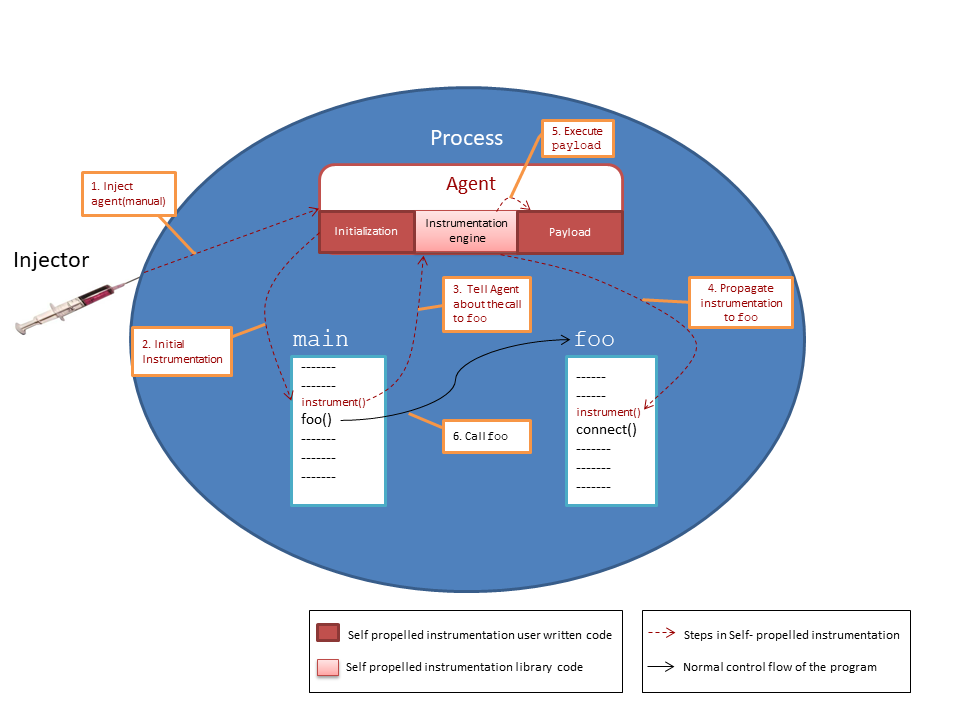
\includegraphics[width=0.90\textwidth]{../user/figure/intraprocess.eps}
  \caption{Intra-process Self-propelled Instrumentation Workflow}
   \label{fig:intrainst}
\end{figure}


Figure~\ref{fig:intrainst} shows an example of intra-process instrumentation
propagation from step 3 to step 5.

In the example, a wrapper function {\em instrument} is invoked right before an
original function call {\em foo}.  The funciton {\em instrument} relies on the
instrumentation engine in the agent library to execute user-provided payload
function and to propagate instrumentation by instrumenting callees inside
function {\em foo}, which include {\em connect} in the example. By this point,
an invocation of {\em instrument} is inserted before {\em connect}. In this way,
instrumentation propagates from a caller to its callees.

\subsubsection{Inter-process propagation}
\begin{figure}[ht]
  \centering
  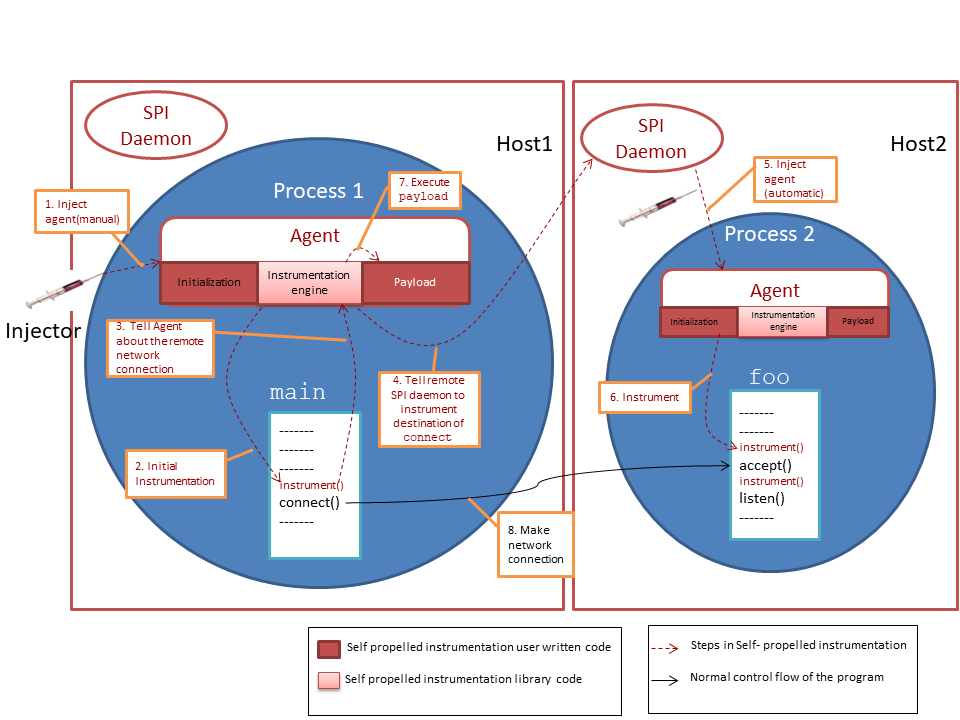
\includegraphics[width=0.90\textwidth]{../user/figure/interprocess.eps}
  \caption{Inter-process Self-propelled Instrumentation Workflow}
  \label{fig:interinst}
\end{figure}

For inter-process instrumentation propagation, the instrumentation engine
identifies communication initiation functions like {\em connect}, {\em send}, or
{\em write} and figures out the remote host.  The instrumentation engine then
contacts to the SPI daemon of the remote host on the other end of communication,
which injects the agent shared library automatically into the target process.
Then the intra-process propagation is performed inside the remote process The
workflow is visualized in Figure~\ref{fig:interinst}

\input{../user/section/4_examples}
\input{../user/section/5_class}

\appendix
\section{Installation}
This appendix describes how to build self-propelled instrumentation
from source code, which can be downloaded from \url{http://www.paradyn.org}
or \url{http://www.dyninst.org}.

Before starting to build self-propelled instrumentation, you have to make sure
that you have already installed and built Dyninst (refer Appendix D in Dyninst
Programming
Guide\footnote{\url{http://www.dyninst.org/sites/default/files/manuals/dyninst/dyninstProgGuide.pdf}
} for building Dyninst).

Building self-propelled instrumentation on Linux platforms is a very simple
three step process that involves: unpacking the self-propelled instrumentation
source, configuring and running the build.

\subsection{Getting the source}
Self-propelled instrumenation`s source code is packaged in \textit{tar.gz}
format. If your self-propelled instrumentation source tarball is called
\textit{src\_spi.tar.gz}, then you could extract it with the commands
\textit{gunzip src\_spi.tar.gz ; tar -xvf src\_spi.tar}. This will create a list
of directories and files.

\subsection{Configuration}
After unpacking, the next thing is to set SP\_DIR, DYNINST\_ROOT, PLATFORM and
DYNLINK variables in \textit{config.mk}.  DYNINST\_ROOT should be set to path of
the directory that contains subdirectories like dyninstAPI, parseAPI etc.,
i.e. within dyninst directory SP\_DIR should be set to the the path of the
current working directory (where self-propelled instrumentation is
installed).

DYNLINK should be set \textit{true} for building agent as a small shared library
that relies on other shared libraries. Otherwise, set DYNLINK as \textit{false}
for buidling a single huge shared library that static-linked all libraries

PLATFORM should be set to one of the following values depending upon what
operating system you are running on:
\begin{table}[h]
\begin{tabular}{l c l}
 i386-unknown-linux 2.4  & : & Linux 2.4/2.6 on an Intel x86 processor \\
 x86\_64-unknown-linux2.4&: &Linux 2.4/2.6 on an AMD-64/Intel x86-64  processor \\
\end{tabular}
\end{table}

Before building, you should also check whether LD\_LIBRARY\_PATH environment
variable is set. If you are using bash shell, then open ~/.bashrc file and check
if LD\_LIBRARY\_PATH is already present. If not, then LD\_LIBRARY\_PATH variable
should be set in a way that it includes {\$DYNINST\_ROOT}/lib directories.  If
you are using C shell, then do the above mentioned tasks in ~/.cshrc file.

If you want to use inter-process propagation, then you should also set the
environment variable SP\_AGENT\_DIR to be the full path of the agent shared
library that will be injected on every machine involved.
 
\subsection{Building}
Once config.mk is set, you are ready to build self-propelled
instrumentation. Move to PLATFORM directory and execute the command
\textit{make}. This will build libagent.so, injector, test-cases and
test-programs. Other make commands for custom building are as follows:

\begin{itemize}
\item make spi: build injector and libagent.so.
\item make injector\_exe: build injector.
\item make agent\_lib: build libagent.so.
\item make unittest: build unittests.
\item make mutatee: build simple mutatees.
\item make external\_mutatee: build real world mutatees, including unix core
  utilities and gcc.
\item make test: equivalent to make unittest + make mutatee + make
  external\_mutatee
\item make clean\_test: clean test stuffs.
\item make clean: only clean core self-propelled stuffs, excluding dependency.
\item make clean\_all: clean everything, including dependency.
\item make clean\_objs: clean core self-propelled objs.
\end{itemize}

That is it! Now, you are all set to use Self propelled intrumentation.


\bibliographystyle{abbrv}
\bibliography{../developer/ref}

\end{document}
